\onehalfspacing

%%CAPITOLO 2: =======================================

\chapter{Word cloud statiche}

Questo capitolo consiste in una breve introduzione al concetto di word cloud.

Nel paragrafo \ref{wc_stat:def} verranno introdotte alcune definizioni e si parler� brevemente di qualche applicazione, mentre nel paragrafo \ref{wc_stat:sem} si far� il punto sullo stato dell'arte riguardo le word cloud semantiche.

\section{Definizioni e applicazioni}\label{wc_stat:def}
\subsection{Cos'� una word cloud?}
Il recente sviluppo di Internet, con l'avvento del Web 2.0, assieme al grande progresso tecnologico dei calcolatori, ha comportato un'ingente produzione di dati sul web e sulle piattaforme web based, per cui il problema di estrarre, gestire e visualizzare efficacemente tale informazione � diventata, negli ultimi anni, un'area di ricerca piuttosto importante nella visualizzazione dell'informazione. 

In generale, una \textbf{word cloud} � una rappresentazione visuale di documenti testuali, che utilizza diversi colori, font e dimensioni per raffigurare le parole pi� rilevanti, dette \textbf{keywords}, di un generico documento. Esse sono utilizzate, quindi, per esaminare un testo, in modo da facilitarne la comprensione, o per confrontare pi� testi. Ad esempio, nelle elezioni presidenziali del 2008 e del 2012 (fig. \ref{fig:obama_romney}), i media americani hanno confrontato le word cloud generate dai dibattiti dei candidati alla presidenza americana, mettendo in risalto le differenze tra i discorsi dei candidati; anche in Italia, in occasione del discorso di insediamento alla Camera da parte del presidente Mattarella, alcune testate giornalistiche hanno fatto uso delle word cloud per analizzare il contenuto del discorso. 
\begin{figure}
\centering
\subfigure[Word cloud generata dal discorso di Obama.]
{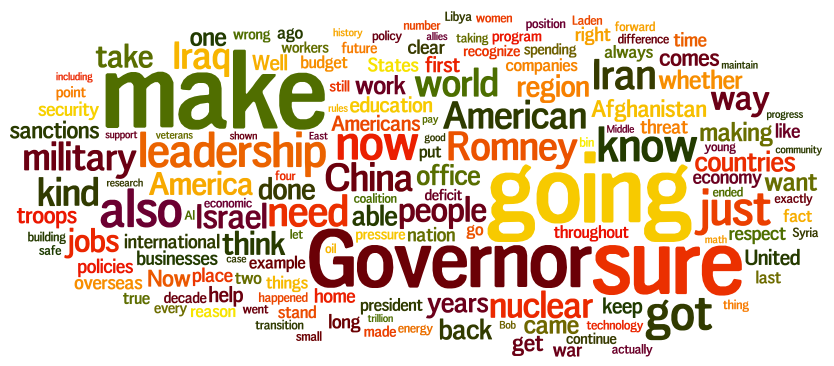
\includegraphics[scale=0.5]{img/wc_statiche/obama_wc.png}}
\hspace{3mm}
\subfigure[Word cloud generata dal discorso di Romney.]
{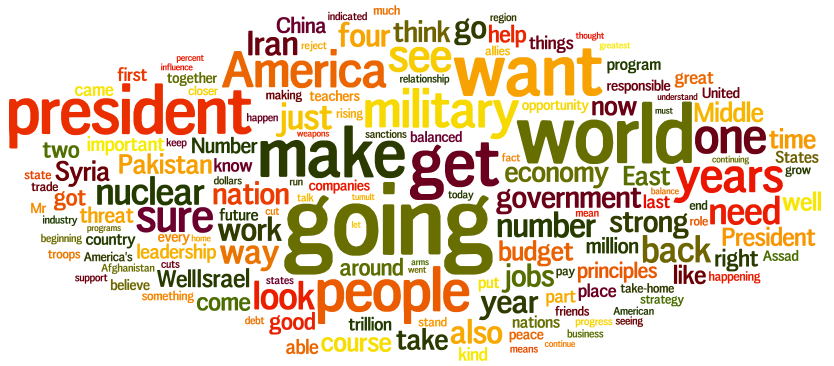
\includegraphics[scale=0.5]{img/wc_statiche/romney_wc.png}}
\caption[Due word cloud relative ai dibattiti tra i candidati alla presidenza statunitense.]{Due wordcloud relative ai dibattiti tra i candidati alla presidenza statunitense.}
\label{fig:obama_romney}
\end{figure}

In riferimento al web, si parla invece di \textbf{tag cloud}, con evidente richiamo ai tag, ovvero ai metadati che riassumono il contenuto di un sito internet. Ogni tag, rappresenta un link ad una specifica risorsa sul web, consentendo agli utenti di accedervi tramite l'utilizzo di keywords. Il loro utilizzo si � diffuso grazie al sito di \textit{photo sharing} Flickr\cite{flickr}, in cui i tag classificano in diverse categorie le foto che vengono condivise tra gli utenti.

Le parole di una word cloud sono tipicamente pesate in base all'importanza che esse ricoprono nel testo: pi� le parole hanno un font grande, pi� sono rilevanti. In questo modo, le word cloud permettono immediatamente di evidenziare ci� che � rilevante in un testo. Ci sono anche altri parametri da tenere in considerazione. In \cite{halvey}, Halvey et al. hanno valutato l'effetto di alcuni fattori: la posizione delle parole, la loro disposizione secondo l'ordine alfabetico e, come detto, la dimensione del font, si sono rivelati essere parametri importanti. Inoltre, hanno notato che gli utenti, piuttosto che leggere tutte le parole, danno uno sguardo generale alla word cloud. In un altro lavoro, Lohmann et al.\cite{Lohmann} hanno scoperto che parole posizionate vicino al centro catturano di pi� l'attenzione rispetto a parole vicine ai bordi, cos� come parole posizionate in alto a sinistra vengono percepite prima delle altre da parte degli utenti.

\subsection{Applicazioni}
Esistono diversi strumenti per la creazione di word cloud. Un tool web based molto popolare, Wordle\cite{Viegas:2009}, grazie alle qualit� grafiche e alle sue funzionalit�, ha permesso la diffusione delle word cloud come potente strumento per riassumere e analizzare un testo. Con Wordle, ad esempio, � possibile impostare alcuni parametri in modo da personalizzare la word cloud finale, come il numero delle parole, il colore, gli angoli di disegno ecc.. Tuttavia, Wordle non riesce a catturare le relazioni semantiche tra le parole, propriet� che pu� rivelarsi cruciale nell'analisi e nella comprensione di un testo. 
Per ovviare a ci�, � stato proposto un ulteriore strumento, basato su Wordle, chiamato ManiWordle\cite{kohk}, il quale offre un buon livello di interazione con l'utente, permettendo a quest'ultimo di manipolare il disegno finale e di modificare le parole visualizzate in termini di posizione, colore e orientamento, risultando quindi pi� flessibile di Wordle. Un altro sistema, SparkClouds\cite{lee}, tramite l'uso delle \textit{sparklines}, mette in risalto i cambiamenti tra pi� word cloud. Collins et al.\cite{collins}, hanno presentato Parallel Tag Clouds, uno strumento in grado di visualizzare le differenze tra i testi scritti di un ricco dataset. FacetAtlas\cite{facetatlas}, invece, � un'applicazione che, tramite grafici e mappe di densit�, visualizza le relazioni che intercorrono tra i documenti di una vasta collezione di testi.

In generale, dunque, negli anni, sono state sviluppate varie applicazioni che generano word cloud, ognuna con pregi e difetti, le quali permettono di comparare diversi documenti da pi� prospettive. Il nostro lavoro � in direzione di quello che � il trend degli ultimi tempi, cio� quello di creare word cloud semantiche, in cui la disposizione delle parole riflette la loro correlazione semantica.

\section{Word cloud semantiche}\label{wc_stat:sem}
Recentemente, la maggior parte dei tool che generano word cloud si � posta come obiettivo quello di raggruppare semanticamente le parole estratte, utilizzando tecniche di elaborazione del linguaggio naturale per correlare parole simili tra loro. Infatti, la possibilit� di disegnare, vicine nella word cloud, parole correlate semanticamente, pu� migliorare l'esperienza dell'utente, come notato da Deutsch et al. in \cite{Deutsch}.

Tree Cloud\cite{gambette}, ad esempio, � un applicazione in cui le parole vengono disposte secondo un albero, in modo tale da preservare la loro vicinanza semantica. In \cite{cui}, Cui et al., tramite misure di similarit�, mirano a collocare, vicine nel disegno, parole correlate semanticamente, utilizzando poi un metodo force directed per compattare la word cloud. Wu et al.\cite{seam}, utilizzano una tecnica ispirata al \textit{seam carving} per ottenere una word cloud semantica e compatta. Questo lavoro di tesi, invece, prende spunto dal recente lavoro svolto da Kobourov et al.\cite{kobourov}, in cui vengono implementati due nuovi algoritmi di visualizzazione, da confrontare con altri algoritmi esistenti, per analizzare la qualit� delle word cloud in base a diverse metriche, ovviamente partendo dalla base comune costituita dalla coerenza semantica nella disposizione delle parole. 